%\subsection{Schema generale: addestramento degli algoritmi di predizione interno a Grafana con estensioni}
%\begin{figure}[H]
%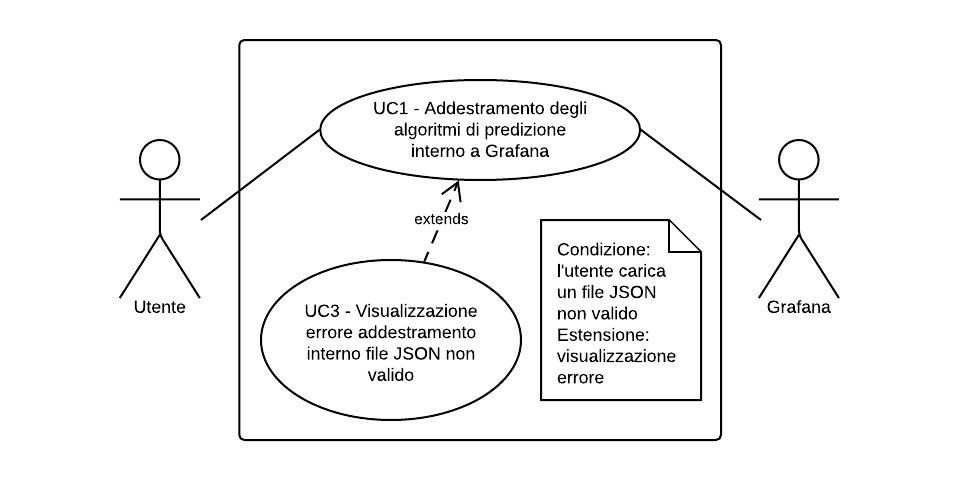
\includegraphics{img/UC1 - Schema generale.png}
%\caption{Schema generale: addestramento degli algoritmi di predizione interno a Grafana con estensioni}
%\end{figure}
\subsection{UC1 - Addestramento degli algoritmi di predizione interno a Grafana}
\begin{figure}[H]
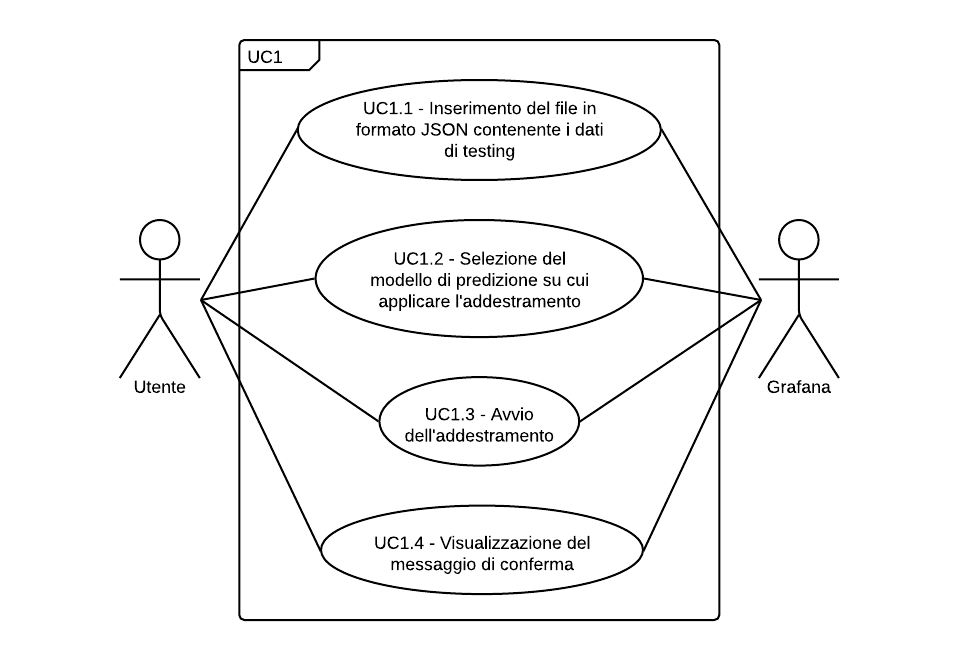
\includegraphics{img/UC1 - Addestramento degli algoritmi di predizione interno a Grafana.png}
\caption{Diagramma degli use case di UC1}
\end{figure}
\begin{itemize}
	\item \textbf{Codice identificativo}: UC1;
	\item \textbf{Titolo}: addestramento degli algoritmi di predizione interno a Grafana\glo;
	\item \textbf{Attori primari}: utente;
	\item \textbf{Attori secondari}: Grafana\glo;
	\item \textbf{Descrizione}: attività di addestramento degli algoritmi di predizione interna a Grafana\glosp utilizzando dei dati inseriti da un utente autenticato;
	\item \textbf{Precondizioni}: l'utente è autenticato nel sistema software Grafana\glo;
	\item \textbf{Postcondizioni}: Grafana\glosp riceve i dati di predizione dopo l'addestramento dei dati caricati da utente;
	\item \textbf{Scenario principale}: 
		\begin{enumerate}
			\item inserimento del file in formato JSON contenente i dati di testing (UC1.1);
			\item selezione del modello di predizione su cui applicare l'addestramento (UC1.2);
			\item avvio dell'addestramento (UC1.3);
			\item visualizzazione del messaggio di conferma (UC1.5).
		\end{enumerate}
	\item \textbf{Scenari alternativi}:
		\begin{enumerate}
			\item arresto dell'addestramento (UC1.4).
		\end{enumerate}
	\item \textbf{Estensioni}:
	\begin{itemize}
		\item se il caricamento del file JSON non è avvenuto con successo viene visualizzato un messaggio di errore (UC3).
	\end{itemize}
\end{itemize}

\subsubsection{UC1.1 - Inserimento del file in formato JSON contenente i dati di testing}
\begin{figure}[H]
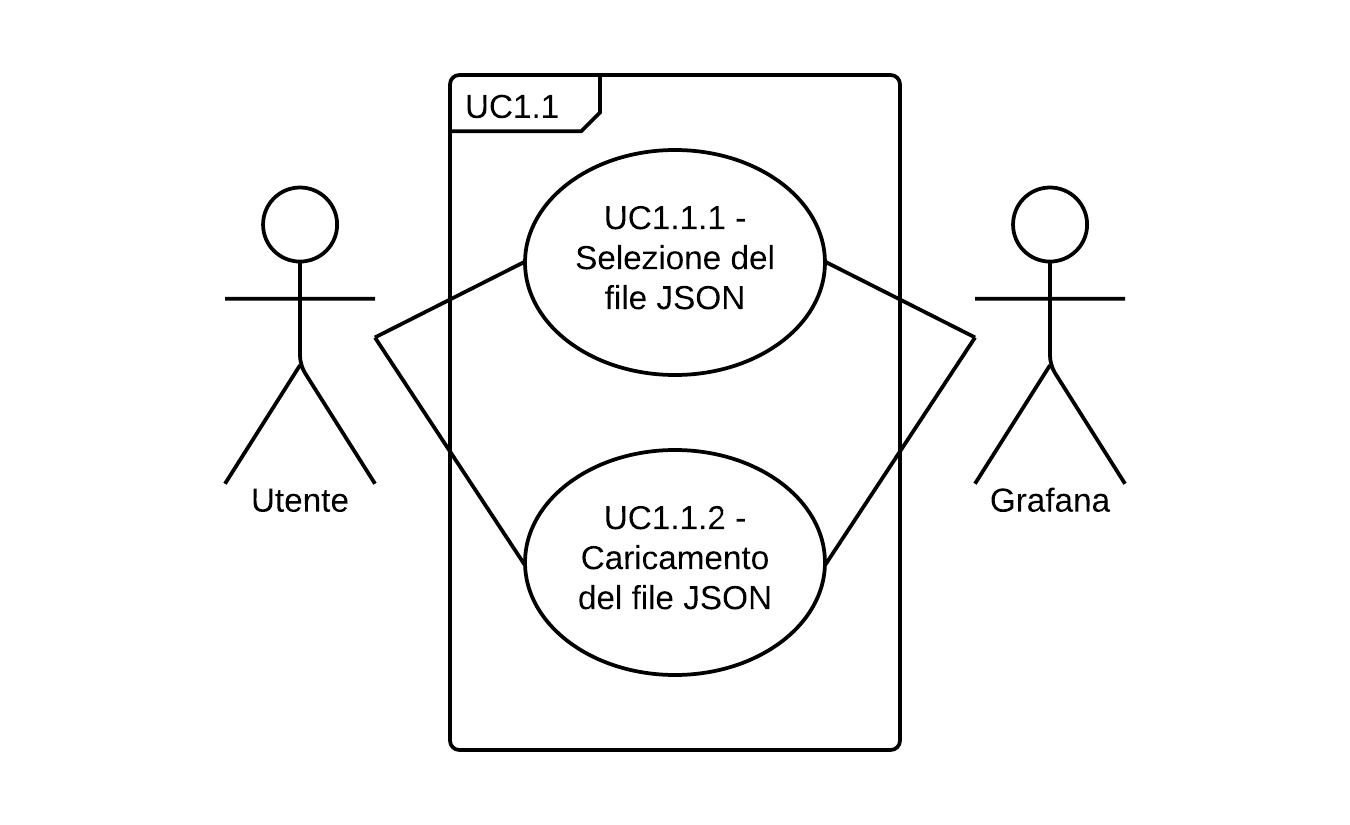
\includegraphics{img/UC1_1_-_Inserimento_del_file_in_formato_JSON_contenente_i_dati_di_testing.png}
\caption{Diagramma degli use case di UC1.1}
\end{figure}
\begin{itemize}
	\item \textbf{Codice identificativo}: UC1.1;
	\item \textbf{Titolo}: inserimento del file in formato JSON contenente i dati di testing;
	\item \textbf{Attori primari}: utente;
	\item \textbf{Attori secondari}: Grafana\glo;
	\item \textbf{Descrizione}: l'utente inserisce nel sistema di Grafana\glosp il file JSON che contiene dati di testing per l'addestramento degli algoritmi di predizione;
	\item \textbf{Precondizioni}: l'utente è autenticato nel sistema software Grafana\glo;
	\item \textbf{Postcondizioni}: il file JSON contenente i dati di testing è stato inserito correttamente;
	\item \textbf{Scenario principale}:
		\begin{enumerate}
			\item selezione del file JSON (UC1.1.1);
			\item caricamento del file JSON (UC1.1.2).
		\end{enumerate}
\end{itemize}
\subsubsection{UC1.2 - Selezione del modello di predizione su cui applicare l'addestramento}
\begin{itemize}
	\item \textbf{Codice identificativo}: UC1.2;
	\item \textbf{Titolo}: selezione del modello di predizione su cui applicare l'addestramento;
	\item \textbf{Attori primari}: utente;
	\item \textbf{Attori secondari}: Grafana\glo;
	\item \textbf{Descrizione}: l'utente seleziona quale modello di predizione applicare durante l'addestramento;
	\item \textbf{Precondizioni}: il file JSON di configurazione è stato inserito correttamente;
	\item \textbf{Postcondizioni}: l'utente ha selezionato correttamente il modello di predizione;
	\item \textbf{Scenario principale}: l'utente seleziona un modello di predizione per eseguire l'addestramento tra SVM\glosp e RL\glo.
	\item \textbf{Specializzazione}:
	\begin{itemize}
		\item selezione del modello di predizione SVM\glosp (UC1.2.1);
		\item selezione del modello di predizione RL\glosp (UC1.2.2).
	\end{itemize}
\end{itemize}
\subsubsection{UC1.2.1 - Selezione del modello di predizione SVM}
\begin{itemize}
	\item \textbf{Codice identificativo}: UC1.2.1;
	\item \textbf{Titolo}: selezione del modello di predizione SVM\glo;
	\item \textbf{Attori primari}: utente;
	\item \textbf{Attori secondari}: Grafana\glo;
	\item \textbf{Descrizione}: l'utente seleziona SVM\glosp come modello di predizione da applicare durante l'addestramento;
	\item \textbf{Precondizioni}: il file JSON di configurazione è stato inserito correttamente;
	\item \textbf{Postcondizioni}: l'utente ha selezionato correttamente SVM\glosp come modello di predizione da applicare;
	\item \textbf{Scenario principale}: l'utente seleziona il modello di predizione SVM\glosp per eseguire l'addestramento.
\end{itemize}
\subsubsection{UC1.2.2 - Selezione del modello di predizione RL}
\begin{itemize}
	\item \textbf{Codice identificativo}: UC1.2.2;
	\item \textbf{Titolo}: selezione del modello di predizione RL\glo;
	\item \textbf{Attori primari}: utente;
	\item \textbf{Attori secondari}: Grafana\glo;
	\item \textbf{Descrizione}: l'utente seleziona RL\glosp come modello di predizione da applicare durante l'addestramento;
	\item \textbf{Precondizioni}: il file JSON di configurazione è stato inserito correttamente;
	\item \textbf{Postcondizioni}: l'utente ha selezionato correttamente RL\glosp come modello di predizione da applicare;
	\item \textbf{Scenario principale}: l'utente seleziona il modello di predizione RL\glosp per eseguire l'addestramento.
\end{itemize}

\subsubsection{UC1.3 - Avvio dell'addestramento}
\begin{itemize}
	\item \textbf{Codice identificativo}: UC1.3;
	\item \textbf{Titolo}: avvio dell'addestramento;
	\item \textbf{Attori primari}: utente;
	\item \textbf{Attori secondari}: Grafana\glo;
	\item \textbf{Descrizione}: l'utente avvia l'addestramento dei dati;
	\item \textbf{Precondizioni}: il file JSON è stato inserito correttamente e il modello di predizione è stato selezionato;
	\item \textbf{Postcondizioni}: l'addestramento è stato avviato con successo;
	\item \textbf{Scenario principale}: l'utente avvia l'addestramento.
\end{itemize}

\paragraph{UC1.4 - Arresto dell'addestramento}
\begin{itemize}
	\item \textbf{Codice identificativo}: UC1.4;
	\item \textbf{Titolo}: arresto dell'addestramento;
	\item \textbf{Attori primari}: utente;
	\item \textbf{Attori secondari}: Grafana\glo;
	\item \textbf{Descrizione}: l'utente arresta l'addestramento prima della sua normale conclusione;
	\item \textbf{Precondizioni}: l'addestramento è stato avviato con successo;
	\item \textbf{Postcondizioni}: l'addestramento è stato fermato con successo;
	\item \textbf{Scenario principale}: l'utente arresta forzatamente l'addestramento.
\end{itemize}

\paragraph{UC1.5 - Visualizzazione del messaggio di conferma}
\begin{itemize}
	\item \textbf{Codice identificativo}: UC1.5;
	\item \textbf{Titolo}: visualizzazione del messaggio di conferma;
	\item \textbf{Attori primari}: utente;
	\item \textbf{Attori secondari}: Grafana\glo;
	\item \textbf{Descrizione}: l'utente visualizza un messaggio di conferma che l'addestramento è stato eseguito correttamente;
	\item \textbf{Precondizioni}: l'addestramento è stato concluso con successo secondo il suo normale flusso di esecuzione;
	\item \textbf{Postcondizioni}: l'utente ha visualizzato un messaggio di conferma che l'addestramento è stato eseguito correttamente;
	\item \textbf{Scenario principale}: l'utente visualizza un messaggio di conferma che l'addestramento è stato eseguito correttamente.
\end{itemize}
